\documentclass[12pt]{article}

\usepackage[T1]{fontenc}
\usepackage[utf8]{inputenc}
\usepackage{newtxtext,newtxmath}
\usepackage[margin=1in]{geometry}
\usepackage{graphicx}
\usepackage{subcaption}
\usepackage{booktabs}
\usepackage{amsmath}
\usepackage{siunitx}
\usepackage{setspace}
\usepackage{parskip}
\usepackage[font=small,labelfont=bf]{caption}
\usepackage[colorlinks, urlcolor=blue, linkcolor=black, citecolor=blue]{hyperref}
\usepackage[numbers,sort&compress]{natbib}

\graphicspath{{figures/}}
\setstretch{1.15}
\sisetup{detect-all}

\title{Fixed-geometry DFT and fine-tuned MACE screening of local lithium energetics in defective graphene and Si$_4$--graphene motifs}

\author{Yuran Chai$^1$ and Xiao Huang$^{2,*}$}
\date{}

\begin{document}

\maketitle
\begin{center}
    \textit{$^1$Department of Chemistry, Wake Forest University, Winston-Salem, NC 27109, USA;\\
    $^2$Department of Chemistry, Duke University, Durham, NC 27708, USA}\\
    $^*$Corresponding author: Xiao Huang
\end{center}

\begin{abstract}
Defects in graphene and local Si--C motifs can alter Li adsorption energetics, but fixed-geometry energy scans and short molecular dynamics trajectories cannot by themselves establish Li migration barriers, diffusion coefficients, or practical anode performance. We therefore revise the present study as a conservative workflow checkpoint: spin-polarized DFT labels are used to fine-tune a MACE-MP-0 foundation model for local Li--C--Si configurations, and the resulting model is diagnosed against the unfine-tuned foundation model, a small three-seed committee, and unwrapped-coordinate LAMMPS trajectories. The dataset contains 273 frames from pristine graphene, monovacancy graphene, divacancy graphene, Stone--Wales graphene, and a model Si$_4$--graphene motif. Independent held-out evaluation shows that fine-tuning reduces the all-family test force RMSE from 285.2 to 20.1 meV \AA$^{-1}$, although the all-family energy RMSE remains 39.1 meV atom$^{-1}$ because of a Si$_4$--graphene family offset. Three fine-tuning seeds complete successfully and give validation force RMSE values of 48.4--107.2 meV \AA$^{-1}$. Unwrapped 400 K NVT simulations over five structures and three velocity seeds complete 100 ps without lost atoms, NaNs, or LAMMPS errors, but their MSD slopes remain short-window diagnostics rather than converged diffusion coefficients. The DFT path scans reveal local endpoint energy differences and path roughness, not activation barriers; final migration-barrier claims require the ongoing relaxed CI-NEB calculations. These results define which parts of the DFT--MACE workflow are currently defensible for local energy and stability screening, and which kinetic claims must remain withheld until the NEB calculations and longer diffusion statistics are complete.
\end{abstract}

\section{Introduction}

Lithium-ion batteries motivate continued study of carbon and silicon-containing negative-electrode materials, but atomistic calculations must distinguish local adsorption descriptors from electrochemical anode performance \citep{tarascon2001issues,obrovac2014alloy}. Graphite remains the commercial benchmark anode, whereas graphene and graphene-derived carbons offer excellent electronic conductivity and tunable defect chemistry that can modify local Li adsorption and migration behavior \citep{novoselov2004electric,yoo2008graphene}. A single-Li model on one graphene sheet is therefore best viewed as a dilute-limit local chemistry model. It cannot directly establish capacity, voltage, rate capability, cycle life, Li--Li clustering, multilayer transport, electrode--electrolyte effects, or Si alloying behavior.

The specific local problem considered here is already close to a substantial first-principles literature. Li adsorption and diffusion on graphene, graphene edges, vacancies, divacancies, and Stone--Wales defects have been examined with DFT and, in some cases, relaxed NEB calculations \citep{uthaisar2010edge,zhou2012graphene,yildirim2014defect}. These studies show that defects can strengthen Li binding and reshape local diffusion paths, but they also demonstrate why endpoint energy differences are not activation barriers. In pristine graphene, for example, the physically relevant hollow-to-hollow path passes through a bridge-like saddle point and has a barrier on the order of several tenths of an eV, not a few hundredths of an eV \citep{uthaisar2010edge,zhou2012graphene}. First-principles studies of Li nucleation further caution that isolated Li adsorption on graphene is not automatically stable against clustering or metallic Li formation \citep{liu2014nucleation}. For Si-containing materials, realistic anode behavior additionally involves Li--Si alloying, large volume changes, and microstructural degradation \citep{obrovac2014alloy,lin2021silicongraphene,martin2019siliconflg}. The Si$_4$--graphene motif used here is consequently a local compositional motif, not a full silicon--graphene composite anode model.

Machine-learned interatomic potentials (MLIPs) can make finite-temperature sampling more affordable once their training domain and uncertainty are controlled \citep{behler2016perspective,jacobs2025mlipguide}. MACE uses higher-order equivariant message passing to build accurate force fields \citep{batatia2022mace}, and MACE-MP-0 provides a broadly trained foundation model for materials chemistry \citep{batatia2025foundation}. Fine-tuning such a model can be useful for a target chemical domain, especially when parts of the foundation representation are kept near their pretrained values \citep{radova2025finetuning}. Related Li--C MLIP work, including Gaussian approximation potentials for Li intercalation in carbon nanostructures, also shows that model validation must be targeted to the intended downstream physics \citep{fujikake2018gap}.

The purpose of this revised manuscript is therefore narrower than the first-draft title implied. We do not claim converged Li mobility, diffusion coefficients, or anode performance. Instead, we document a rapid DFT--MACE workflow for local Li--C--Si energy screening, report the parts that pass basic diagnostic checks, and identify the specific calculations needed to convert this workflow into a defensible kinetic study.

\section{Method}

\subsection{Model systems}

Five model systems were constructed with the Atomic Simulation Environment (ASE) \citep{larsen2017ase}: pristine graphene, monovacancy graphene, divacancy graphene, Stone--Wales graphene, and a Si$_4$--graphene motif. The starting cell was a 5 $\times$ 5 graphene supercell with approximately 15 \AA{} of vacuum normal to the sheet. A monovacancy was generated by removing one central C atom, and a divacancy was generated by removing a nearest-neighbor C--C pair. The Stone--Wales model was generated by rotating a central C--C bond in the initial graphene lattice. The Si-containing system contains four Si atoms placed above graphene and should be described as a Si$_4$--graphene motif, not as a general Si--graphene composite. A Li atom was placed near the central adsorption region of each structure. Figure~\ref{fig:structures} defines the model families.

\begin{figure}[!t]
  \centering
  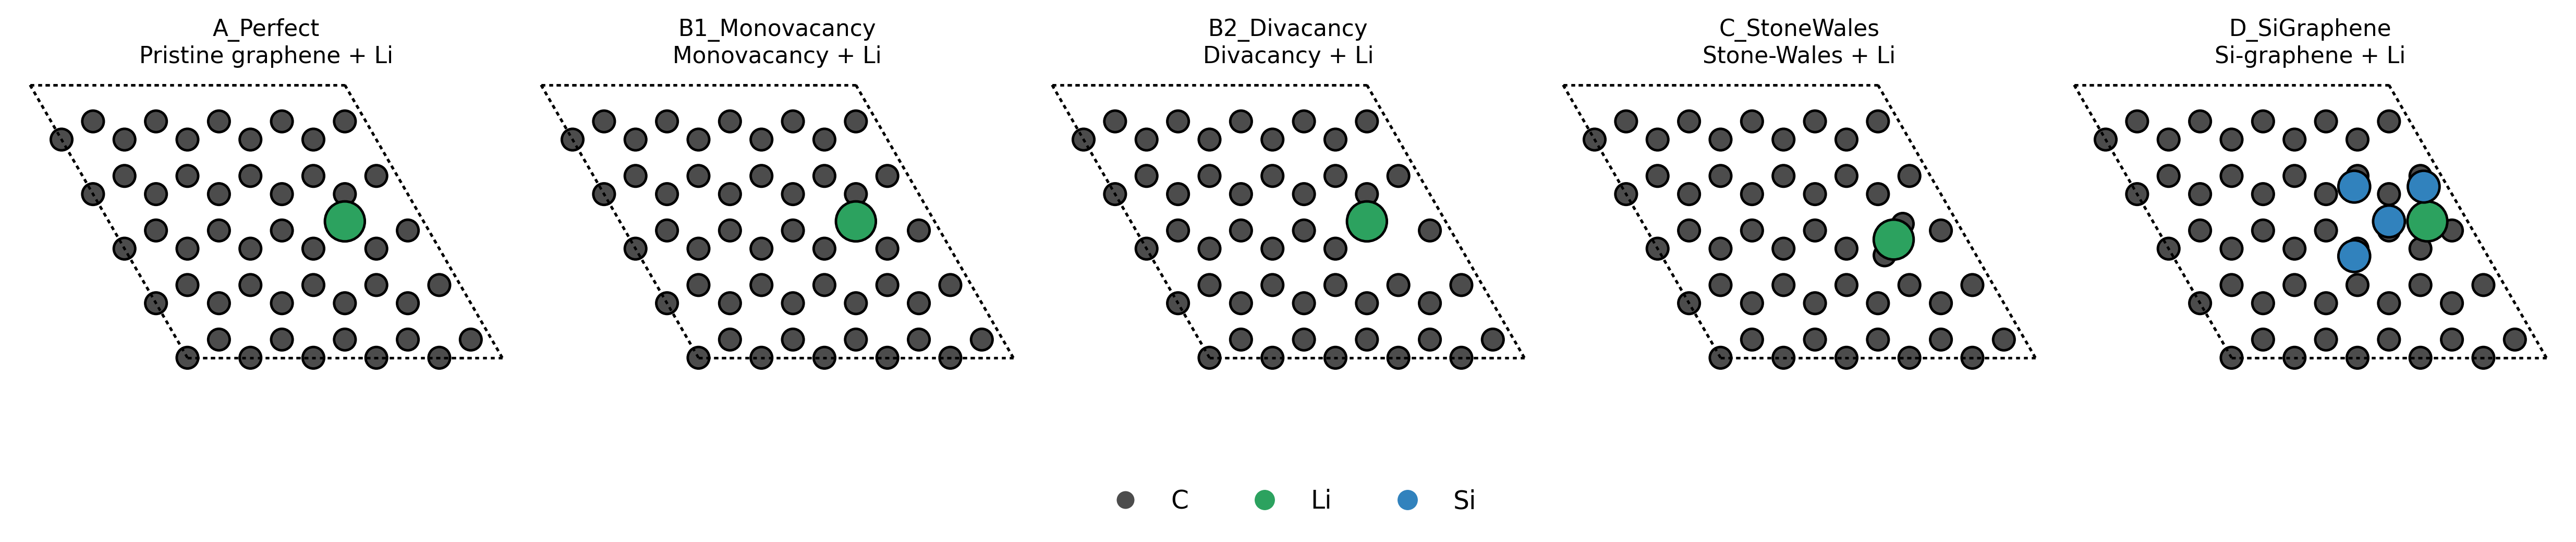
\includegraphics[width=\textwidth]{structure_models.png}
  \caption{Initial local structure families used for DFT labeling and MACE diagnostics: pristine graphene, monovacancy graphene, divacancy graphene, Stone--Wales graphene, and a Si$_4$--graphene motif. Carbon, lithium, and silicon atoms are shown in gray, green, and blue, respectively. The figure is a structural identifier; publication-quality defect zooms and relaxed final structures should be added before journal submission.}
  \label{fig:structures}
\end{figure}

\subsection{DFT labeling}

DFT calculations were performed with VASP \citep{kresse1996efficient,kresse1996cms} using PAW potentials \citep{blochl1994paw,kresse1999paw} and the PBE exchange--correlation functional \citep{perdew1996pbe}. The calculations used spin polarization, ENCUT = 520 eV, a Gamma-centered 3 $\times$ 3 $\times$ 1 k-point mesh, Gaussian smearing with ISMEAR = 0 and SIGMA = 0.05 eV, LASPH = .TRUE., ADDGRID = .TRUE., and ISYM = 0. Ionic relaxations used IBRION = 2, NSW = 100, EDIFF = $10^{-5}$ eV, and EDIFFG = -0.02 eV \AA$^{-1}$. Single-point site and path-scan labels used NSW = 0 and EDIFF = $10^{-6}$ eV. The present labels did not include an explicit vdW correction or dipole correction. This omission is important because Li adsorption on graphitic surfaces and one-sided slab adsorbates can be sensitive to both effects; a final kinetic study should repeat the key labels with PBE-D3 or another tested dispersion treatment and slab dipole correction \citep{grimme2010d3}.

The final MACE dataset contains 273 frames: 194 frames from ionic relaxation trajectories and 79 fixed-geometry site/path single-point calculations. Site labels sample the initial Li position, hollow-like sites, bridge-like sites, top-like sites, and Si$_4$-related positions. Path labels are linear Cartesian interpolation images between two sampled endpoints. No climbing-image NEB calculation was performed \citep{henkelman2000neb}. Consequently, the path quantities below are reported as fixed-geometry path-scan descriptors and endpoint energy differences. They should not be called migration barriers.

\subsection{MACE fine-tuning and validation}

The DFT-labeled structures were converted to extended XYZ files and split into 211 training frames, 31 validation frames, and 31 held-out test frames. The split is deterministic but not ideal: interpolation images from the same path can remain highly correlated across splits, so the validation and test errors are same-workflow diagnostics rather than strong transferability metrics. The MACE-MP-0 medium foundation model \citep{batatia2025foundation} was fine-tuned with a force-heavy objective using energy and force weights of 1.0 and 100.0. Embedding and interaction learning-rate factors were set to zero, while product and readout layers remained trainable; stochastic weight averaging was used in the second stage. This learning-rate-factor strategy avoids hard-coding a layer index for freezing the foundation-model backbone.

The first draft reported only validation error. Here we report held-out test errors, family-specific test errors, and a direct comparison with the unfine-tuned MACE-MP-0 foundation model. A three-member committee was also trained with different random seeds to estimate the sensitivity of the small-data fine-tuning procedure. These diagnostics are still limited by the small and correlated dataset, but they directly address whether fine-tuning improves the target Li--C--Si force predictions relative to the foundation model.

\subsection{Short molecular dynamics diagnostics}

LAMMPS \citep{plimpton1995lammps} simulations used the converted MACE model with the MACE pair style. The small structures were replicated 2 $\times$ 2 $\times$ 1 for short MD diagnostics, producing 196--220 atoms depending on defect family. This replication also replicates Li and defects; for example, the pristine 2 $\times$ 2 $\times$ 1 cell contains four Li atoms, not one Li atom. This artificial periodic concentration must be considered when interpreting any Li displacement.

Reviewer-response trajectories were run at 400 K for 100 ps with a 1 fs timestep and three independent velocity seeds for each structure. Coordinates were dumped with unwrapped Li positions or image-flag-consistent quantities, and Li in-plane MSD traces were post-processed from the unwrapped coordinates. We report these trajectories as short-window stability and displacement diagnostics only. They are not long enough to produce converged diffusion coefficients, and the replicated small cells are not a concentration-converged model of a realistic electrode.

\section{Results and Discussion}

\subsection{Training diagnostics and held-out errors}

The dataset spans five distinct defect and compositional environments (Fig.~\ref{fig:mace_error}a). Under the independent post-training evaluator, the fine-tuned model reduces the held-out all-family test force RMSE from 285.2 meV \AA$^{-1}$ for the unfine-tuned MACE-MP-0 foundation model to 20.1 meV \AA$^{-1}$ (Fig.~\ref{fig:mace_error}b and Table~\ref{tab:mace_errors}). This 92.9\% force-error reduction demonstrates that fine-tuning is necessary for the present Li--C--Si labels. Energy errors improve more modestly, from 50.0 to 39.1 meV atom$^{-1}$ on the all-family test split, because the Si$_4$--graphene family has a systematic energy offset while retaining low force error. The force-error gap across train, validation, and test splits still indicates that the model should not be treated as broadly transferable beyond the labeled structural domain.

\begin{figure}[!t]
  \centering
  \begin{subfigure}{0.44\textwidth}
    \centering
    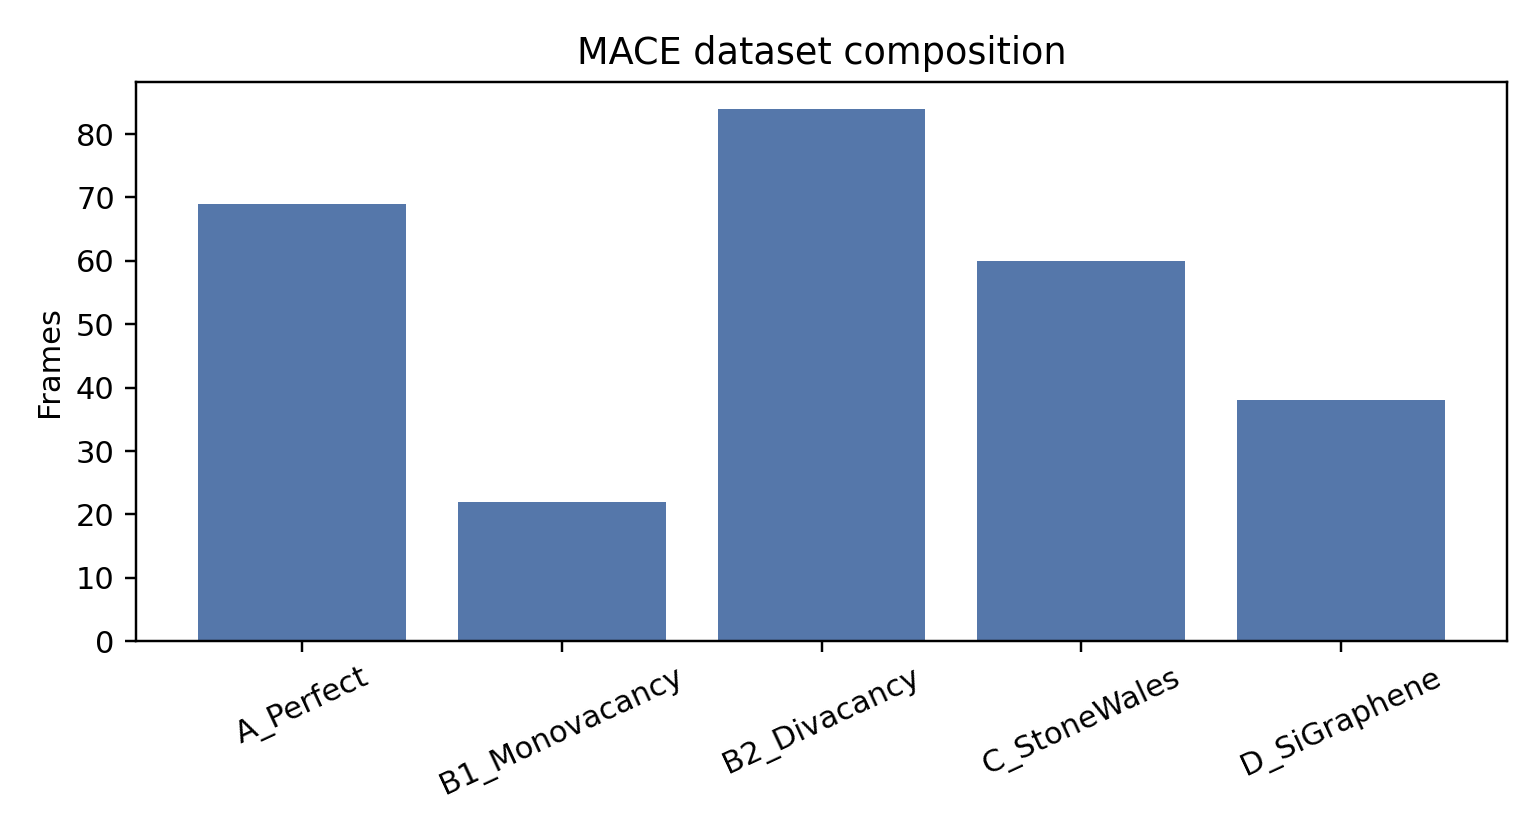
\includegraphics[width=\textwidth]{dataset_family_counts.png}
    \caption{Frame counts by family.}
  \end{subfigure}
  \hfill
  \begin{subfigure}{0.52\textwidth}
    \centering
    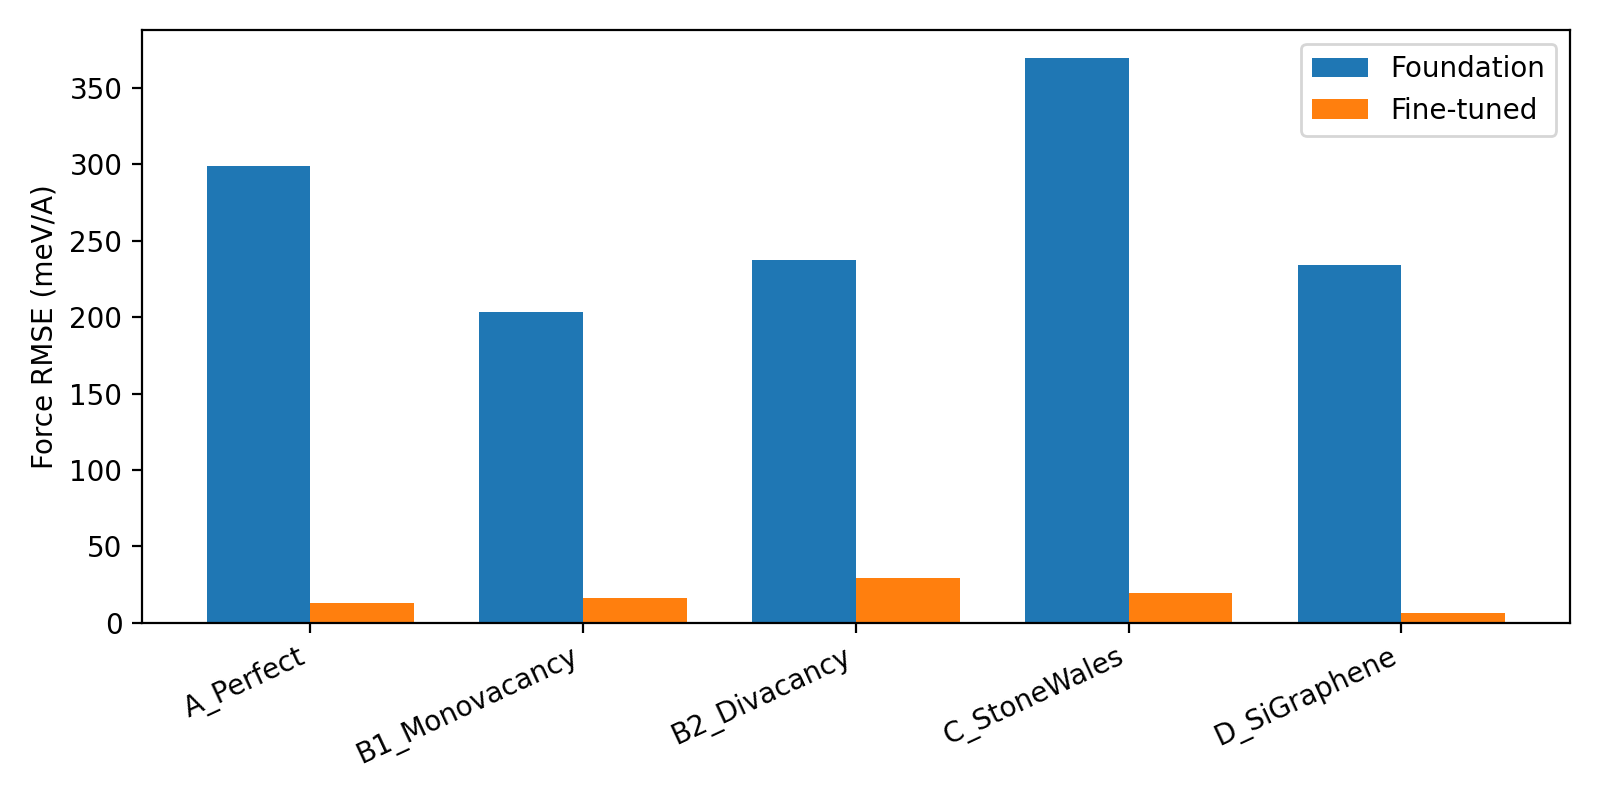
\includegraphics[width=\textwidth]{review_mace_foundation_comparison.png}
    \caption{Foundation-model versus fine-tuned held-out test force RMSE.}
  \end{subfigure}
  \caption{MACE dataset and reviewer-response error diagnostics. Fine-tuning strongly reduces held-out force error relative to the unfine-tuned MACE-MP-0 foundation model. The small and correlated split design still limits transferability claims, especially for finite-temperature defect reconstruction.}
  \label{fig:mace_error}
\end{figure}

\begin{table}[!t]
  \centering
  \caption{Independent MACE evaluator diagnostics. Force RMSE is reported as frame-level RMS force error.}
  \label{tab:mace_errors}
  \begin{tabular}{lcc}
    \toprule
    Model and split or family & Energy RMSE (meV atom$^{-1}$) & Force RMSE (meV \AA$^{-1}$) \\
    \midrule
    Foundation, test all & 50.0 & 285.2 \\
    Fine-tuned, training all & 41.2 & 10.3 \\
    Fine-tuned, validation all & 39.2 & 39.0 \\
    Fine-tuned, test all & 39.1 & 20.1 \\
    Fine-tuned test: pristine graphene & 5.3 & 12.7 \\
    Fine-tuned test: monovacancy graphene & 5.2 & 16.3 \\
    Fine-tuned test: divacancy graphene & 2.8 & 29.3 \\
    Fine-tuned test: Stone--Wales graphene & 3.5 & 19.3 \\
    Fine-tuned test: Si$_4$--graphene motif & 108.3 & 6.8 \\
    \bottomrule
  \end{tabular}
\end{table}

The three-member fine-tuning committee also completed successfully. The seed-dependent validation force RMSE values are 96.4, 107.2, and 48.4 meV \AA$^{-1}$ for seeds 20260427, 20260428, and 20260429, respectively. The spread is a useful uncertainty warning for the small dataset: the fine-tuned potential is clearly better than the foundation baseline for this target domain, but individual finite-temperature trajectories should still be interpreted with model-coverage caution. These values support interpolation within the present labeled structures but do not validate high Li concentration, Li clustering, or real Si--graphene composite lithiation.

\subsection{Fixed-geometry site energetics}

The fixed-geometry site scan identifies relative energies among the sampled Li placements (Fig.~\ref{fig:energy_landscape}a). Pristine graphene favors the hollow C$_3$ site among the sampled positions. Monovacancy, divacancy, and Si$_4$--graphene motifs have the initial Li position as the lowest sampled site. This should not be overinterpreted: a ``prior Li'' minimum can indicate a real local trap, but it can also indicate that the search grid is too sparse or that the initial placement biased the sampled site set. In the Stone--Wales structure, the top-C site is lowest within this fixed-geometry scan; because prior literature emphasizes the importance of relaxed defect geometry, this result should be treated as provisional until relaxed adsorption-site searches are completed \citep{zhou2012graphene,yildirim2014defect}.

\begin{figure}[!t]
  \centering
  \begin{subfigure}{0.43\textwidth}
    \centering
    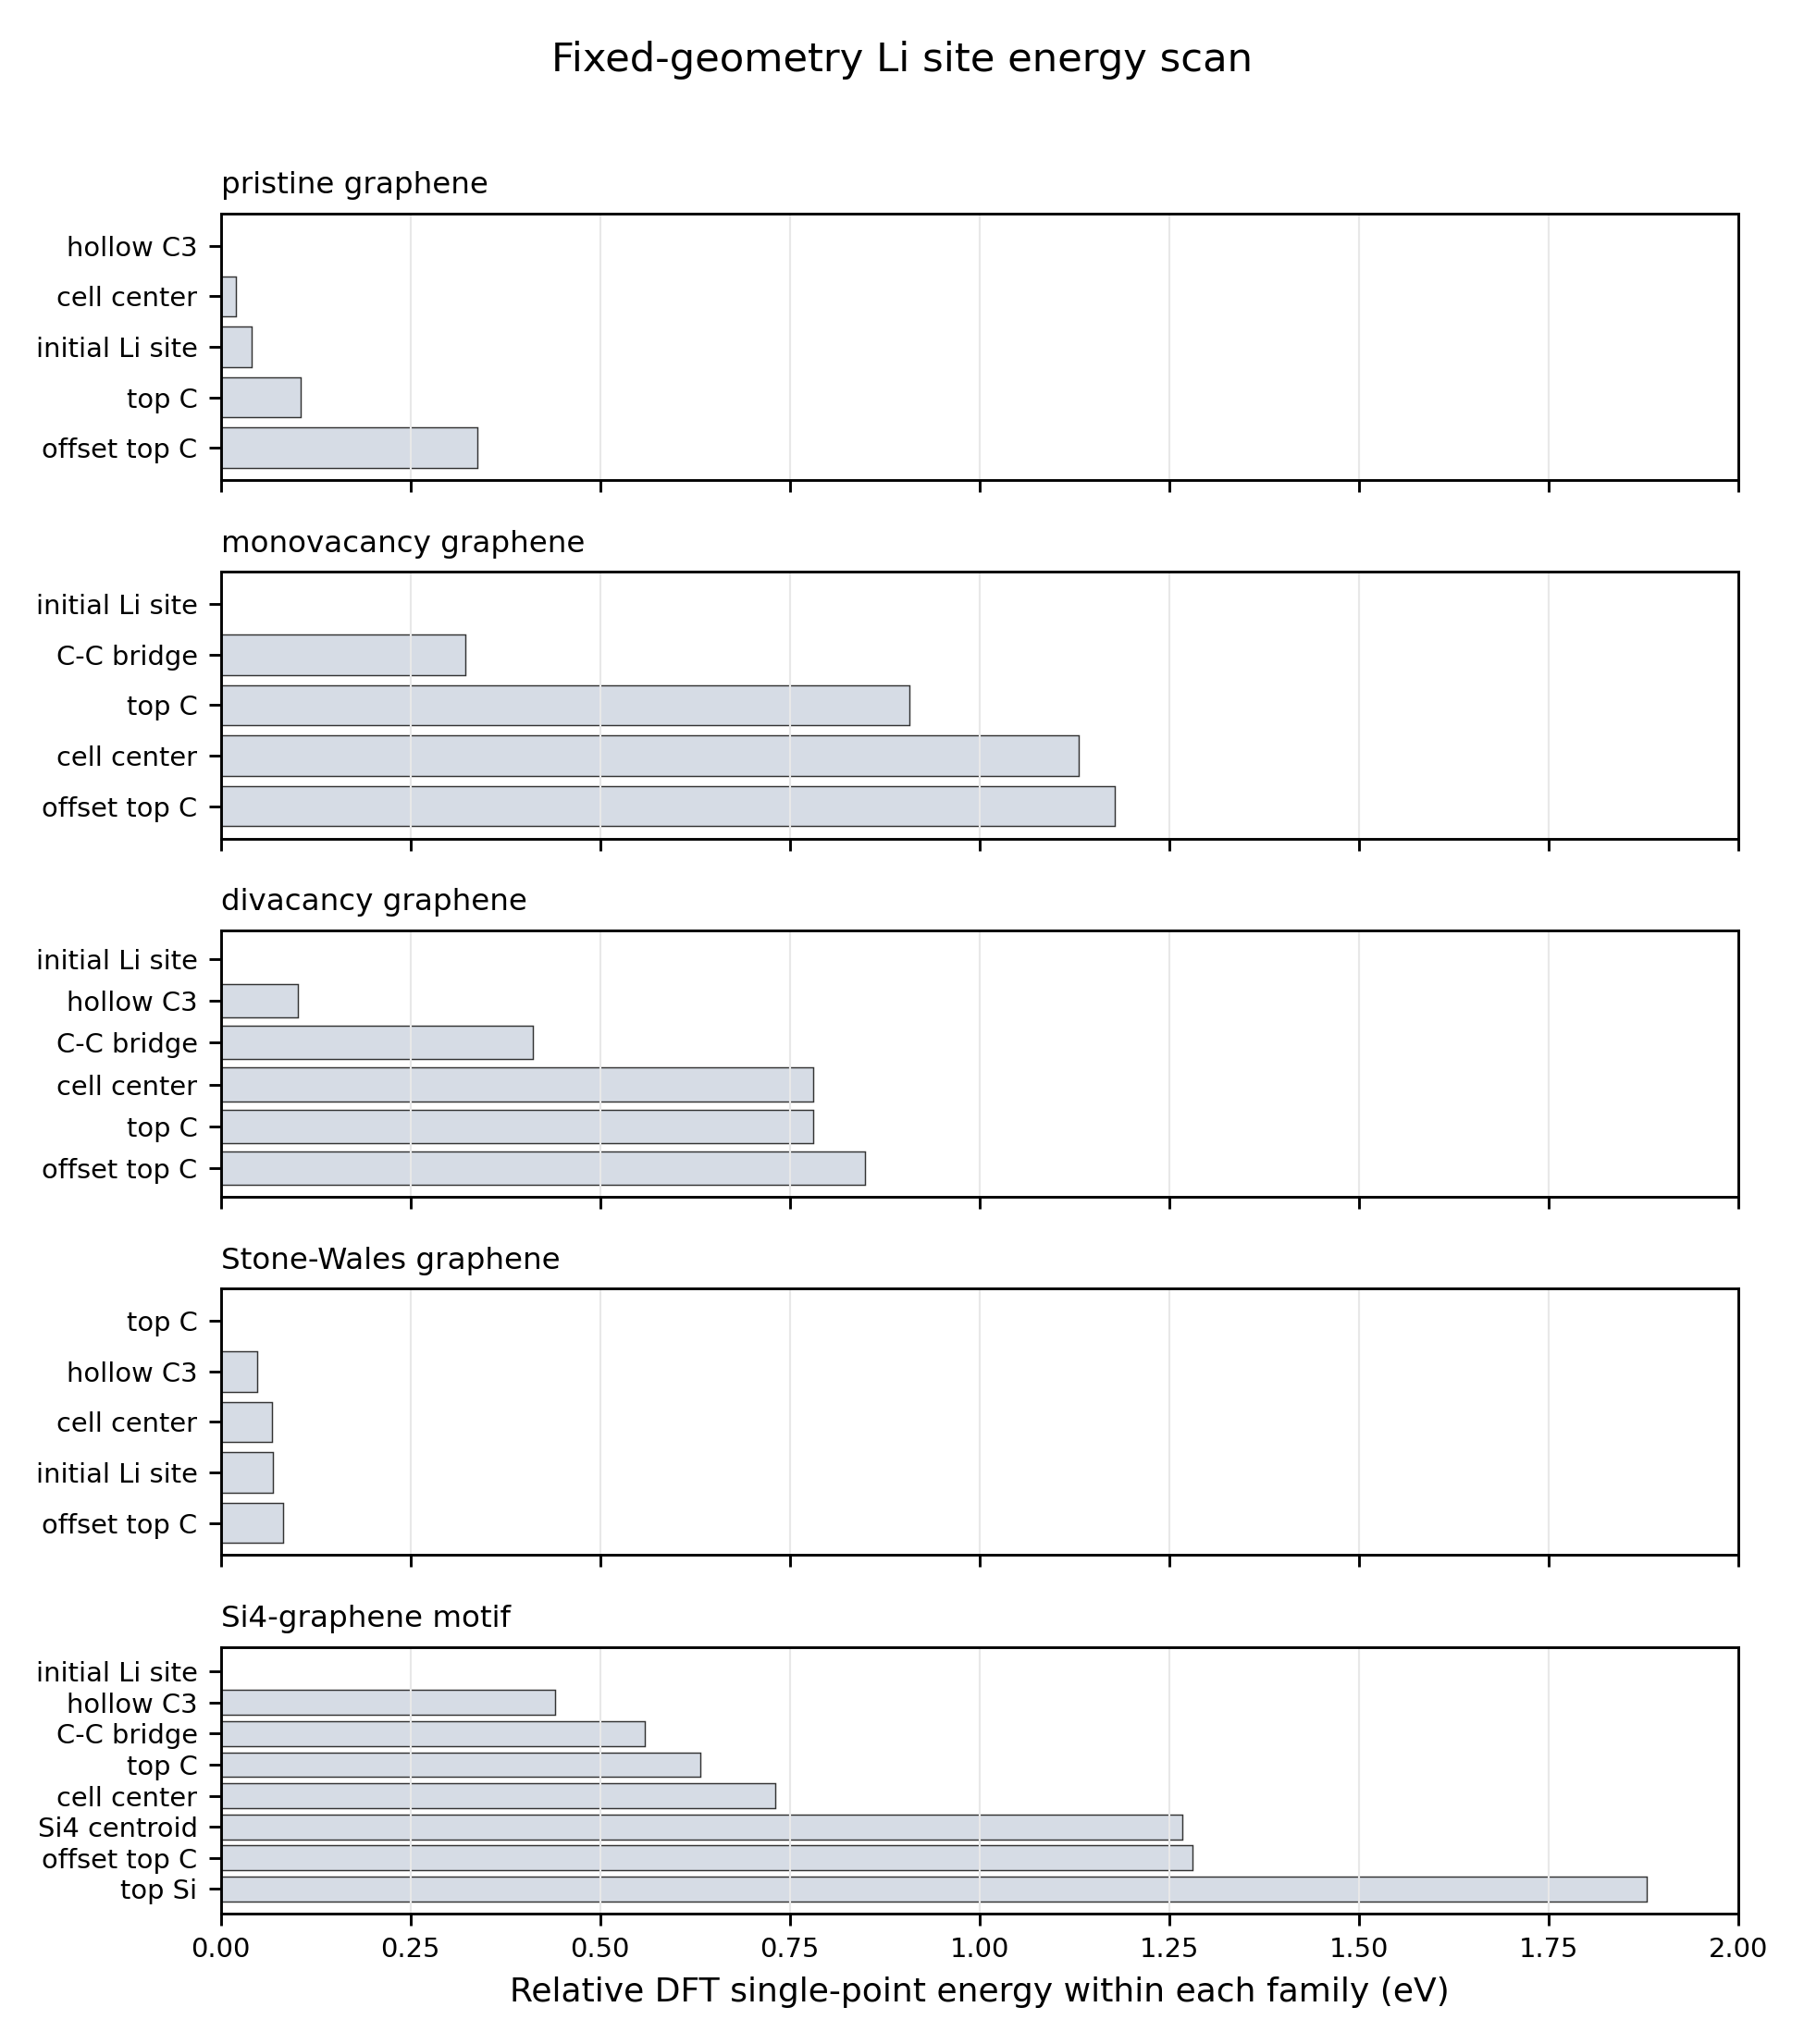
\includegraphics[width=\textwidth]{site_energy_rankings_revised.png}
    \caption{Site energy scan with a common energy scale.}
  \end{subfigure}
  \hfill
  \begin{subfigure}{0.54\textwidth}
    \centering
    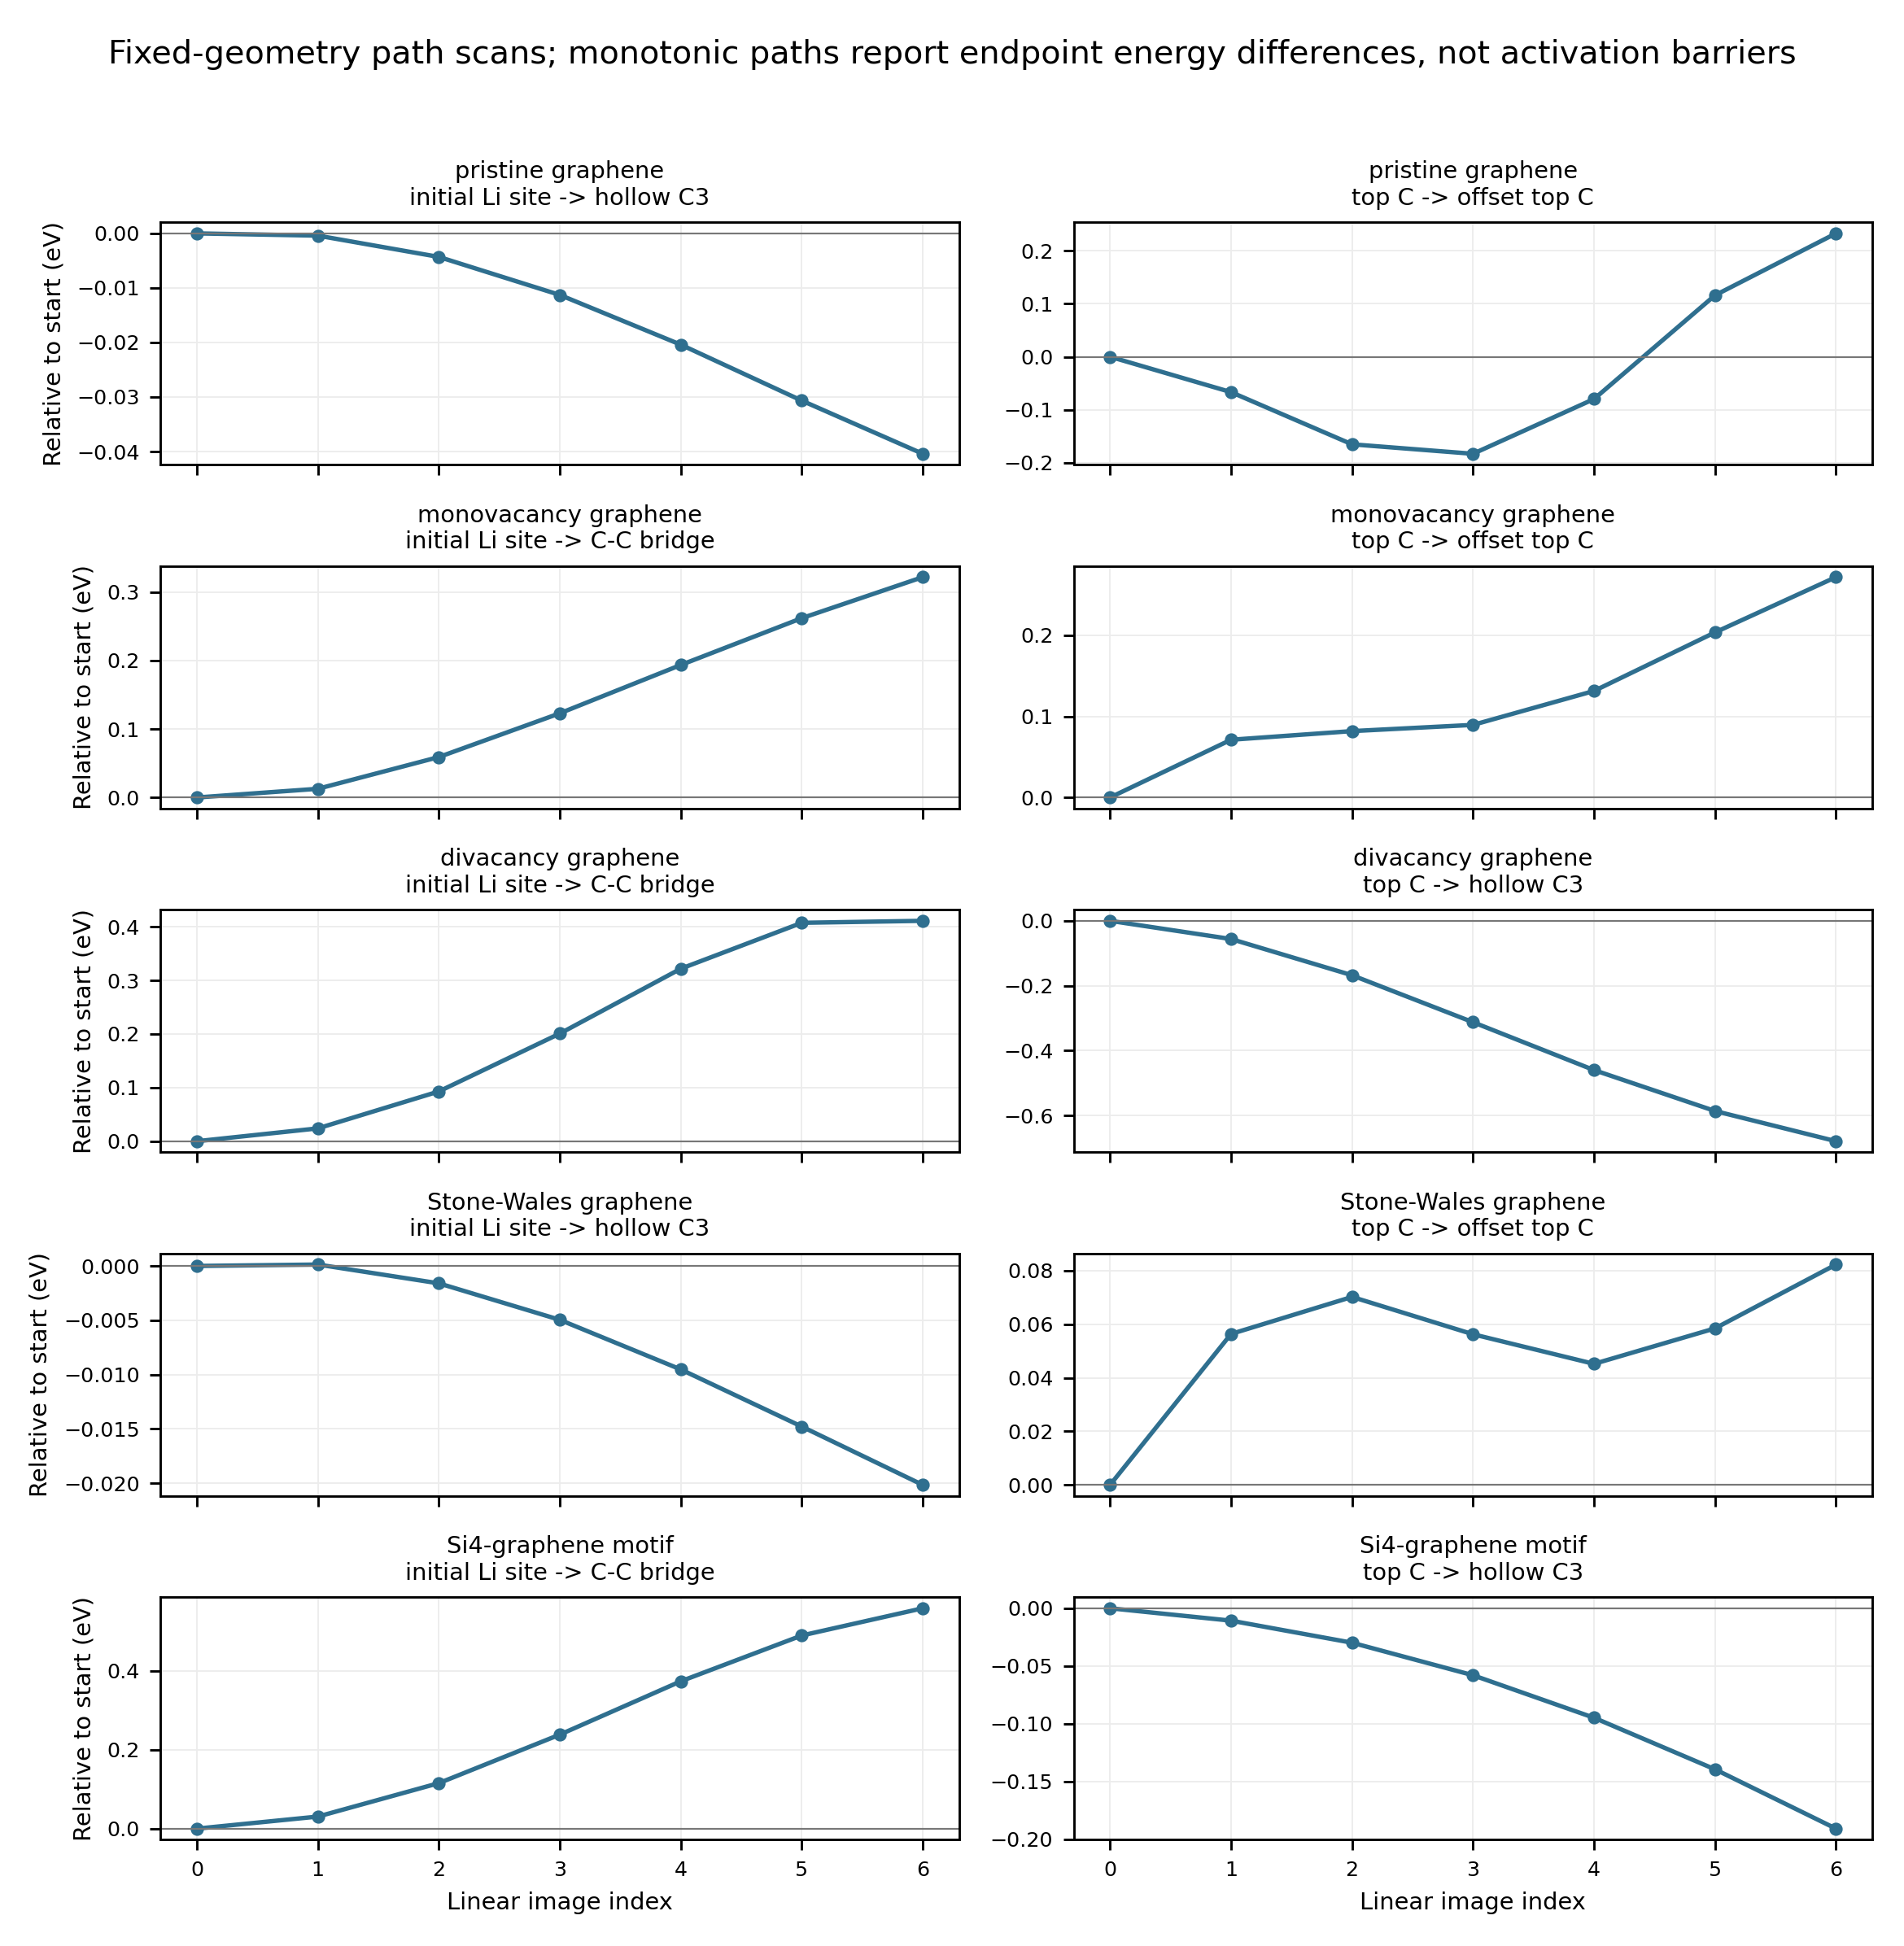
\includegraphics[width=\textwidth]{path_profiles_revised.png}
    \caption{Linear interpolation path scans.}
  \end{subfigure}
  \caption{DFT fixed-geometry energy landscape. These panels show site-energy differences and path roughness on the frozen scan geometries. They do not report relaxed adsorption energies or NEB activation barriers.}
  \label{fig:energy_landscape}
\end{figure}

The main chemically safe statement is therefore qualitative: local defects and Si$_4$ decoration strongly perturb Li site energetics in the sampled geometries. The current data do not establish whether these perturbations improve reversible storage. Strongly binding defect sites may stabilize Li locally, but they can also impede Li migration and potentially promote irreversible trapping.

\subsection{Endpoint energy differences, not migration barriers}

Table~\ref{tab:path_scans} replaces the first draft's ``barrier'' table. For the representative rows criticized in review, the reported path-span values often equal $|\Delta E_{\mathrm{end-start}}|$, which means the path maximum and minimum occur at endpoints. Such paths do not sample an independent saddle point. They are endpoint energy differences or fixed-geometry path spans, not activation barriers.

\begin{table}[!t]
  \centering
  \caption{Fixed-geometry path-scan descriptors. ``Path span'' is the maximum minus minimum single-point energy along the sampled interpolation images; it is not a NEB barrier.}
  \label{tab:path_scans}
  \begin{tabular}{llcc}
    \toprule
    System & Path & Path span (eV) & $\Delta E_{\mathrm{end-start}}$ (eV) \\
    \midrule
    Pristine graphene & initial Li $\rightarrow$ hollow C$_3$ & 0.040 & -0.040 \\
    Pristine graphene & top C $\rightarrow$ offset top C & 0.416 & 0.233 \\
    Monovacancy graphene & initial Li $\rightarrow$ C--C bridge & 0.322 & 0.322 \\
    Monovacancy graphene & top C $\rightarrow$ offset top C & 0.272 & 0.272 \\
    Divacancy graphene & initial Li $\rightarrow$ C--C bridge & 0.411 & 0.411 \\
    Divacancy graphene & top C $\rightarrow$ hollow C$_3$ & 0.680 & -0.680 \\
    Stone--Wales graphene & initial Li $\rightarrow$ hollow C$_3$ & 0.020 & -0.020 \\
    Stone--Wales graphene & top C $\rightarrow$ offset top C & 0.082 & 0.082 \\
    Si$_4$--graphene motif & initial Li $\rightarrow$ C--C bridge & 0.559 & 0.559 \\
    Si$_4$--graphene motif & top C $\rightarrow$ hollow C$_3$ & 0.191 & -0.191 \\
    \bottomrule
  \end{tabular}
\end{table}

This correction changes the scientific interpretation. The 0.040 eV pristine value and 0.020 eV Stone--Wales value cannot be used to claim low Li migration barriers. They are small endpoint downhill energies in the sampled scans. A physically meaningful comparison with the graphene literature requires relaxed hollow--bridge--hollow or equivalent minimum-energy paths, preferably via CI-NEB \citep{uthaisar2010edge,zhou2012graphene,henkelman2000neb}. Until those calculations are completed, this study can only discuss fixed-geometry local energy roughness.

\subsection{Short MD stability diagnostics}

The reviewer-response 400 K NVT trajectories are useful as model diagnostics but not as equilibrium diffusion simulations. All 15 100 ps trajectories (five systems $\times$ three velocity seeds) completed without LAMMPS errors, lost atoms, or NaNs (Table~\ref{tab:md_diagnostics}). This is a substantial improvement over the first-draft wrapped-coordinate 10 ps diagnostic, but it still does not provide converged diffusion coefficients. The unwrapped in-plane Li MSD traces show strong seed-to-seed variability, especially for the Si$_4$--graphene motif (Fig.~\ref{fig:md_diag}).

\begin{figure}[!t]
  \centering
  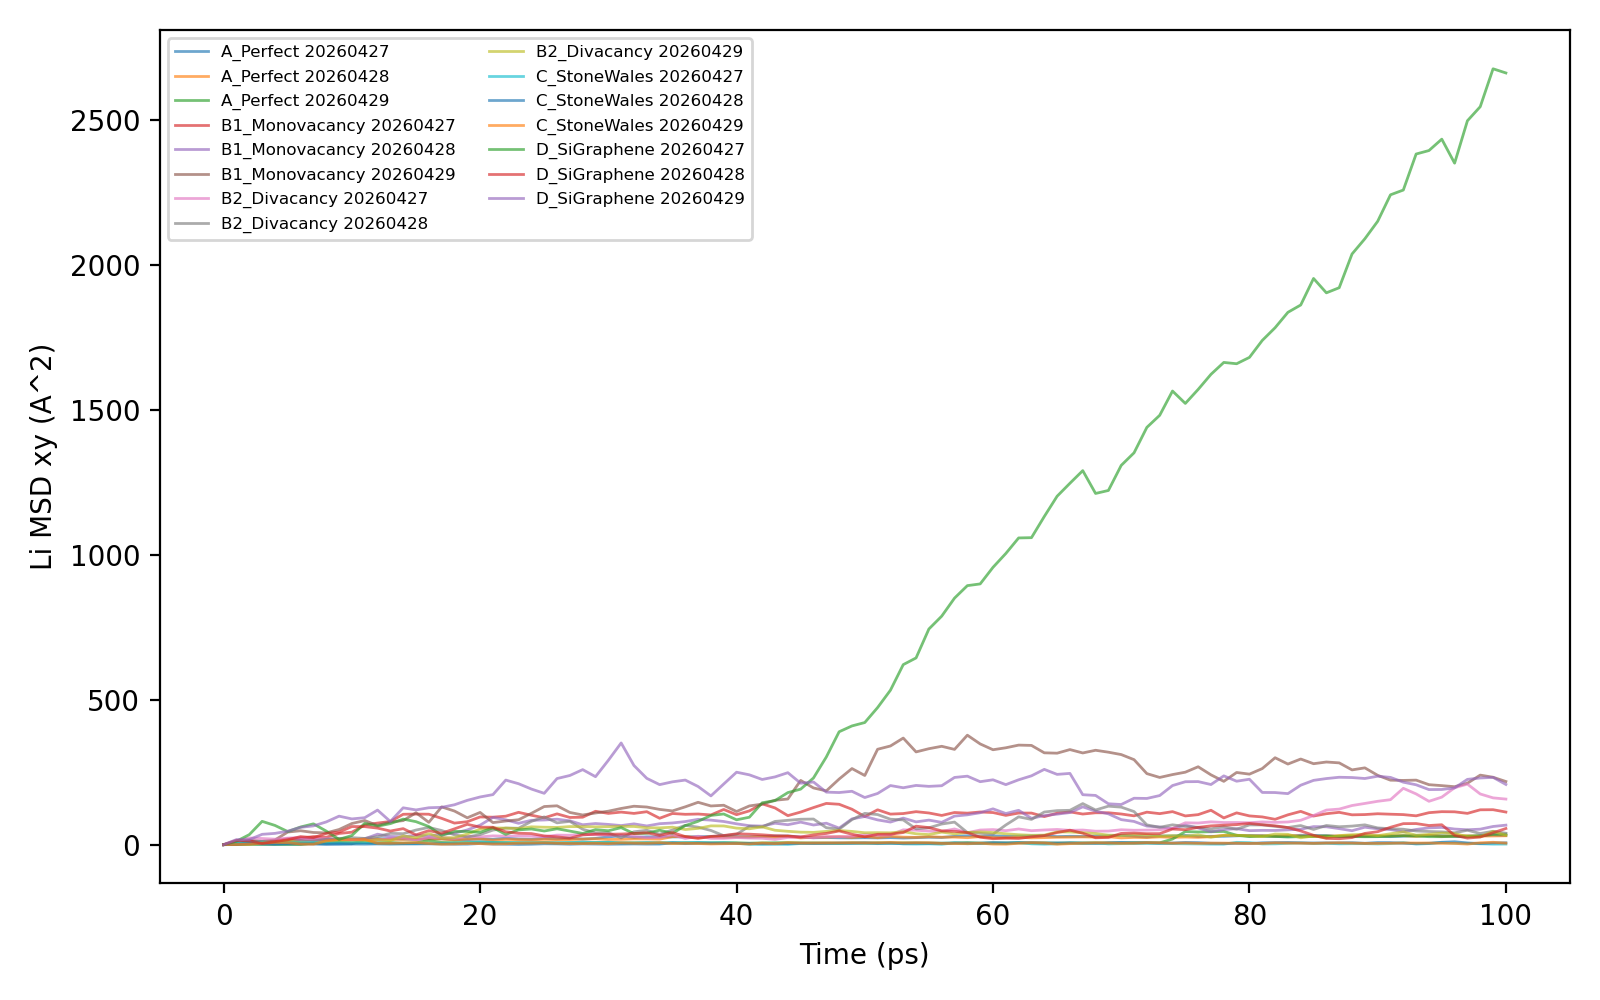
\includegraphics[width=0.92\textwidth]{review_md_unwrapped_msd_xy_traces.png}
  \caption{Unwrapped-coordinate Li in-plane MSD traces from 100 ps, 400 K NVT reviewer-response trajectories. These curves diagnose short-window displacement behavior and stability only. They are not long enough, and the cells are not large or dilute enough, to report converged diffusion coefficients.}
  \label{fig:md_diag}
\end{figure}

\begin{table}[!t]
  \centering
  \caption{400 K, 100 ps unwrapped-coordinate MACE/LAMMPS diagnostics. Short-window $D_{xy}$ is obtained from the 20--100 ps linear-slope diagnostic and is not a converged diffusion coefficient.}
  \label{tab:md_diagnostics}
  \begin{tabular}{lccc}
    \toprule
    System & Seeds completed & Final MSD$_{xy}$ (\AA$^2$) & Short-window $D_{xy}$ ($10^{-6}$ cm$^2$ s$^{-1}$) \\
    \midrule
    Pristine graphene & 3/3 & $32.8 \pm 3.1$ & $5.6 \pm 4.0$ \\
    Monovacancy graphene & 3/3 & $132.5 \pm 77.2$ & $13.6 \pm 31.9$ \\
    Divacancy graphene & 3/3 & $76.4 \pm 70.0$ & $12.1 \pm 30.0$ \\
    Stone--Wales graphene & 3/3 & $4.5 \pm 2.3$ & $0.25 \pm 1.31$ \\
    Si$_4$--graphene motif & 3/3 & $974.8 \pm 1462.3$ & $299 \pm 518$ \\
    \bottomrule
  \end{tabular}
\end{table}

The key interpretation is conservative. Stable program completion and unwrapped-coordinate MSD traces show that the fine-tuned model can run short reviewer-response trajectories across all five structural families. However, several curves remain non-linear over 100 ps, and one Si$_4$--graphene seed dominates the apparent displacement scale. These data should therefore be reported as stability and displacement diagnostics, not as final Li diffusivities or mechanistic proof of fast Si$_4$--graphene transport. Additional longer trajectories, larger cells, independent Li concentrations, and DFT checks of representative high-displacement snapshots are still required before quantitative diffusion claims are defensible.

\subsection{Implications and required follow-up}

The revised evidence supports only a limited conclusion: fine-tuned MACE can interpolate the current fixed-geometry DFT labels with modest held-out errors, and the workflow identifies where the current model and sampling protocol are insufficient. It does not yet support statements about Li mobility, diffusion coefficients, rate capability, storage capacity, or mechanical/electronic advantages of Si--graphene anodes.

The minimum calculations needed for a stronger manuscript are now more specific. First, the currently running relaxed CI-NEB paths should be completed and benchmarked against the graphene literature before any migration-barrier language is restored. Second, representative high-displacement MD snapshots, especially from the Si$_4$--graphene seed with the largest MSD, should receive DFT single-point checks to test whether the MACE trajectory remains within the labeled domain. Third, longer trajectories and larger cells are needed to convert the present short-window displacement diagnostics into quantitative diffusivity estimates.

\section{Conclusion}

We revised the Li--MACE graphene study into a conservative local-energy and model-validation manuscript. The current DFT dataset and fine-tuned MACE model are useful for documenting sampled Li site energetics and for demonstrating a large force-error reduction relative to the unfine-tuned MACE-MP-0 foundation model. The three-seed committee and 15 unwrapped 100 ps MD diagnostics strengthen the workflow relative to the first draft. However, the fixed-geometry path scans are not migration barriers, and the short-window MSD diagnostics cannot be sold as converged diffusion coefficients. The Si-containing model should be described as a Si$_4$--graphene local motif rather than a representative silicon--graphene composite anode.

The main outcome is therefore methodological and diagnostic: the workflow is now transparent about its limits and identifies the remaining calculations needed for a defensible kinetic study. A journal-ready article on Li diffusion in defective graphene should add relaxed CI-NEB barriers benchmarked against prior DFT work, DFT validation of high-displacement MD snapshots, and longer/larger-cell MD statistics before restoring quantitative lithium diffusion or battery-performance claims. Until those data are available, the defensible claim is local energy screening plus target-domain MACE validation, not quantitative lithium diffusion or practical anode performance prediction.

\section*{Data and Code Availability}

The scripts, processed CSV files, and generated figures used for this draft are stored in the project workspace under \texttt{/home/xh121/Li-vasp}. A public archival repository and supporting-information package should be prepared before journal submission, including VASP input files, structure coordinates, MACE training commands, LAMMPS input files, model-checkpoint metadata, and post-processing scripts.

\section*{Author Contributions}

Author-contribution details should be finalized before submission.

\section*{Competing Interests}

The authors declare no competing financial interests.

\bibliographystyle{achemso}
\bibliography{references}

\end{document}
